% Created 2021-04-02 Fri 17:39
% Intended LaTeX compiler: pdflatex
\documentclass[11pt]{article}
\usepackage[utf8]{inputenc}
\usepackage[T1]{fontenc}
\usepackage{graphicx}
\usepackage{grffile}
\usepackage{longtable}
\usepackage{wrapfig}
\usepackage{rotating}
\usepackage[normalem]{ulem}
\usepackage{amsmath}
\usepackage{textcomp}
\usepackage{amssymb}
\usepackage{capt-of}
\usepackage{hyperref}
\usepackage{minted}
\usepackage[margin=1in]{geometry}
\usepackage{subcaption}
\author{A. Bochkarev}
\date{}
\title{Facility Location with BDDs: Status update 2}
\hypersetup{
 pdfauthor={A. Bochkarev},
 pdftitle={Facility Location with BDDs: Status update 2},
 pdfkeywords={},
 pdfsubject={},
 pdfcreator={Emacs 28.0.50 (Org mode 9.4.3)}, 
 pdflang={English}}
\begin{document}

\maketitle

\section{Status}
\label{sec:org36e25f4}
\begin{itemize}
\item we are dealing with the Facility location problem in the following edition: every facility can
"cover" all its neighbors, we have to cover every customer at least once, no
overlap costs; we have "colored" facilities + budget for number of locations
per color.
\item I have implemented constructing BDDs for (1) \textbf{cover} constraints, and (2) \textbf{color} constraints.
\item with this problem formulation, intersection BDD is still very large, but now
we have at least something to discuss, as the process depends on \emph{many} factors.
\end{itemize}

\section{The problem.}
\label{sec:org62955c5}
First, let me re-introduce my ``model'' problem. Assume I have the following seven nodes:
\begin{center}
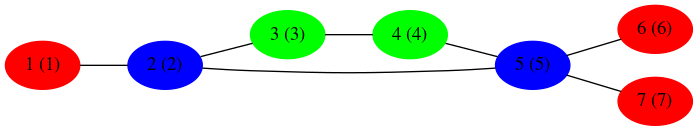
\includegraphics[width=.9\linewidth]{problem_LR.png}
\end{center}

Color limits are as follows: red (5), blue (1), green (3). (So, the point is I
can't have two ``central'' blue nodes \textcircled{2} and \textcircled{5} at the
same time -- other limits are not binding.)

\section{Plan of attack}
\label{sec:org7eb4fef}

\section{The algorithm}
\label{sec:org694daf3}

\subsection{Covering DD}
\label{sec:orge4cdf4e}

\subsection{Color DD}
\label{sec:orgf80870e}

\section{Random instances generation}
\label{sec:org680cb5b}

\section{Some results of numerical modeling.}
\label{sec:orgc5d5017}

\subsection{Diagram sizes (table)}
\label{sec:org3625a65}

\subsection{Runtimes}
\label{sec:org7e85580}

\section{Discussion}
\label{sec:orgda304c8}
\begin{itemize}
\item sorting variables in \texttt{color} diagram.
\item random graph generation (limit node degree?)
\item next node selection in the (cover) BDD generation procedure.
\end{itemize}
\end{document}